\section{Adaptive Filtering}

\subsection{Adaptive FIR Filters \hayes{497}}
\begin{minipage}{8cm}
        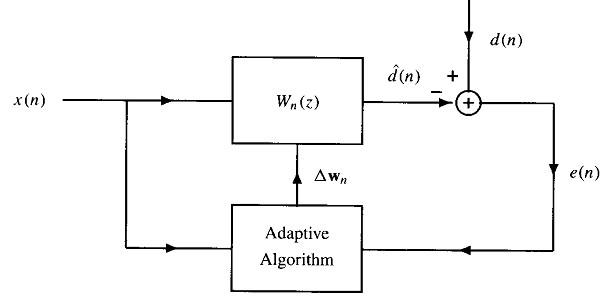
\includegraphics[width=8cm]{./bilder/adaptiveFiltering.jpg}
\end{minipage}
\begin{minipage}{10.5cm}
    \textbf{Goal:} The filter coefficients $w_n$ should be adapted with recursive modification $\Delta w_n$ itself.
    
    \textbf{application area:}
    \begin{liste}
        \item System identification: estimate $H[k], h[n]$ 
        \item Equalize transmission canal  with known sequence: GSM, \ldots
        \item Adaptive noise cancelling (in ear plugs)
        \item Echo cancelling on phone calls
    \end{liste}
\end{minipage}\\
   
The MSE (mean square error) $\xi(w_0, w_1, \ldots, w_n) = E\left(|e(i)|^2\right) = E\left( \left[ d(i) - \sum\limits_{k=0}^{N} w_k x(i-k)\right] ^2 \right)$ should be minimizied. The solution for stationary process is the Wiener-Hopf equations: \\
$$R_x\cdot w = r_{dx}$$
If the process isn't stationary, the filter coefficients have to be updated every step for the optimal result: $w_{n+1}= w_n + \Delta w_n$\\
The adaptive filter should 
\begin{liste}
	\item converge \textbf{to the Wiener-Hopf equations} if the environment is stationary. $\lim\limits_{n\rightarrow\infty} w_n = R_x^{-1}\cdot r_{dx}$
	\item be able to compute the update coefficients $\Delta w_n$, \textbf{without knowledge} of $R_x$ and $r_{dx}$
	\item be able to adapt to the \textbf{changing statistics} and track the solution, if the environment is nonstationary
\end{liste}
\subsubsection{Steepest Descent Adaptive Filter \hayes{499}}
To solve the Wiener-Hopf equations, in every step the autocorrelation matrix has to be inverted and with the crosscorrelation multiplied. 
To reduce this calculations, the coefficient are updated into optimal direction with a small step.
\begin{minipage}{13cm}
$$w_{n+1}=w_n-\mu \cdot  \dfrac{\delta \xi}{\delta w_n} =w_n-\mu \cdot \bigtriangledown\xi(n) \Rightarrow \boxed{ w_{n+1}= w_n+\mu \cdot E\left\lbrace e(n)x^*(n)\right\rbrace}$$
$$ 0<\mu< \frac 2 \lambda_{max}; \lambda_{max} = \text{maximum eigenvalue of autocorrelation matrix } R_x$$
To compute the $E\left\lbrace e(n)x^*(n)\right\rbrace$, a averaging over the last L sample has to be done.  
$$E\left\lbrace e(n)x^*(n)\right\rbrace= \frac{1}{L}\sum\limits_{l=0}^{L-1}e(n-l)x^*(n-l)$$
\end{minipage}
\begin{minipage}{6cm}
        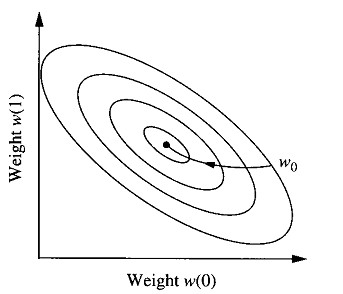
\includegraphics[width=6cm]{../StatDig/bilder/steepestDescent.jpg}
\end{minipage}

\clearpage
\subsubsection{LMS Algorithm \hayes{505}}
\begin{minipage}{14cm}

  The LMS algorithm use the same idea as the steepest descent, but just choose the last sample (L=1).\\
  $\boxed{ w_{n+1}=w_n+\mu \cdot e(n) \cdot x^*(n) }$\\
  
  The LMS just converges in the mean, if $0<\mu< \frac{2}{(p+1)E\left(|x(n)|^2\right)}=\frac{2}{(p+1)r_x(0)}$.
  The filter coefficients converge to $\hat d(n) = d(n)$ or $e(n) = 0$. 
  That means that filter coefficients always will move, but in the mean they are correct.
\end{minipage}
\begin{minipage}{5cm}
  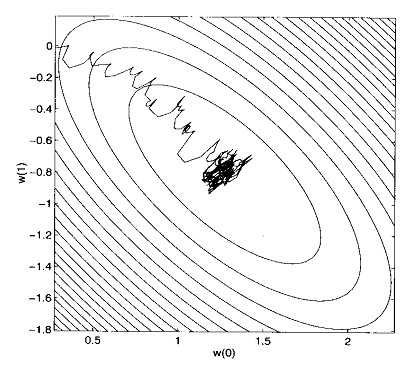
\includegraphics[width=5cm]{../StatDig/bilder/LMS.jpg}
\end{minipage}

\begin{minipage}{9cm}
  \begin{tabbing}
  	Parameters:  \= $p= $ Filter order\\
  	Init:		\> $w_0= 0$\\
  	Computation:
  \end{tabbing}	
      \begin{aufzaehlung}
          \item calculate filter output: $\hat{d}(n) = w_n^T\cdot x(n)$ 
          \item calculate error: $e(n) = d(n) - \hat{d}(n)$
          \item update filter coefficients: $w_{n+1}=w_n+\mu e(n)x^*(n)$  
      \end{aufzaehlung}\vspace{0.05cm}

\end{minipage} 
\begin{minipage}{10cm}
  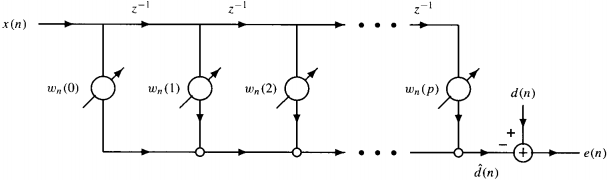
\includegraphics[width=10cm]{../StatDig/bilder/adaptiveFirStructure.png}
\end{minipage}

\subsubsection{Normalized LMS (NLMS) \hayes{514}}
The NLMS is most command used, because it's easy to program, fast to compute and convergence quite fast.\\
The idea is to adapt also the stepsize $\mu(n)=\frac{\beta}{\|x(n)\|^2} \Rightarrow $
$\boxed{w_{n+1}=w_n +\beta \frac{x^*(n)}{\epsilon+\|x(n)\|^2}e(n)}$\\
Where $\|x(n)\|^2$ is the signal power, $\epsilon$ is used for small $\|x(n)\|$ and is a small positive number and $0<\beta<2$.\\\\
To reduce the calculation the normalization term $\|x(n)\|$ can also be calculatet recursively:\\ $\|x(n+1)\|^2 =  \|x(n)\| + |x(n+1)|^2 -|x(n-p)|^2$

\subsubsection{Applications - Noise Cancellation \hayes{517}}
\begin{minipage}{9cm}
        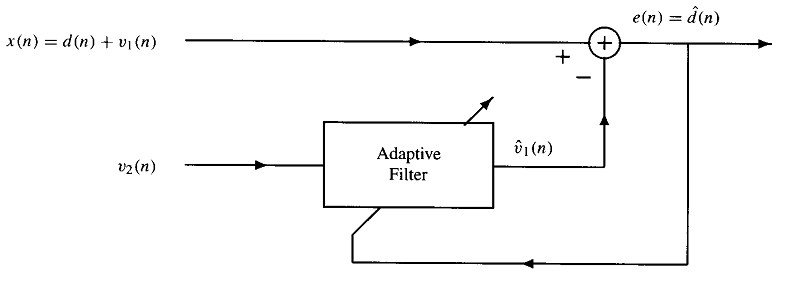
\includegraphics[width=8.5cm]{../StatDig/bilder/adaptiveNoiseCancellation.jpg}\\
        Input signal $x(n)$ with noise (e.g. car noise). 
        The second input measures only the noise (e.g. separate mic). Therefore, $v_1$ and $v_2$ are correlated.
        The filter now guesses the first noise so that the error signal gives the wanted signal $d(n)$.     
\end{minipage}
\hspace{3mm}
\begin{minipage}{9cm}
        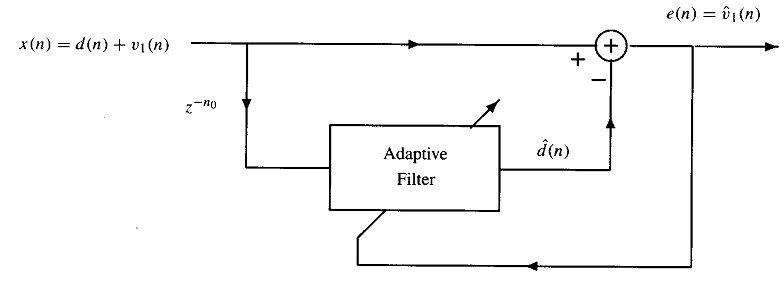
\includegraphics[width=8.5cm]{../StatDig/bilder/NoiseCancellationwithoutRef.jpg}\\
        Input signal $x(n)$ with noise (e.g. car noise). The signal $d(n)$ has to be narrowband and $v_1(n)$ has to be broadband. ($d$ has to be a ``slow''  and $v_1$ has to be a ``fast'' changing signal)
        The filter predicts now $d(n)$ and the error signal is the noise $v_1$.
\end{minipage}

\subsection{Adaptive Recursive Filters (won't be tested) \hayes{534}}
\begin{minipage}{8.4cm}
	Benötigt im Vergleich zum LMS Algorithmus $20M$ nur $2M$ Iterationen bis er konvergiert. RLS nutzt alle vergangene 
	Information zur Berechnung der Korrektur; LMS nutzt nur momentane Information. \\
	$\mathbf{s}(n) = [s(n), s(n-1), \ldots, s(n - N + 1)]^T$ \\
	Forgetting-Faktor ($\mu=1$),
	Initialisierungsfakt. ($\delta = 1)$
\end{minipage}
\begin{minipage}{11cm}
	\begin{aufzaehlung}
	    \item Initialisieren: $n=1; \mathbf{P}(0)=\gamma \cdot \mathbf{I}; \mathbf{\hat{c}}(0)=0$
	    \item Gain Vektor: $ \mathbf{k}(n) = \frac{\mathbf{P}(n-1)\mathbf{s}(n)}{1 + \mathbf{s}^T(n) \mathbf{P}(n-1) \mathbf{s}(n)}$
	    \item Wahrer Schätzfehler: $\eta(n) = r(n) - \mathbf{s}^T(n) \mathbf{\hat{c}}(n-1)$
	    \item Koeffizienten updaten: $\mathbf{\hat{c}}(n) = \mathbf{\hat{c}}(n-1) + \mathbf{k}(n) \eta(n)$
	    \item Fehlerkorrelationsmatrix: \small $\mathbf P(n) = \frac1\mu [ \mathbf P (n-1) - \mathbf k (n) \mathbf u^T (n) \mathbf P(n-1)]$
\normalsize	    \item $n++$ und zurück zu Schritt 2
	\end{aufzaehlung}
\end{minipage}

